\section{Metoder}
\label{ch:metoder}
En kort præsentation af de to mest dominerende arbejdsmetoder der er anvendt.\\

I dette projekt er der anvendt metoder indlært gennem et tidligere projekt. Værktøjerne er de værktøjer som gruppen føler sig trygge ved og som gruppen føler bidrager mest til processen. 
\subsection{Scrum}
I gruppens implementering af Scrum startes der med at lave en produktbacklog, som er den kunden ser.  Derefter planlægges det første sprint. Et sprint spænder over to uger. Når et sprint starter bliver opgaver overført fra backloggen til sprintet. Her bliver omfanget af opgaven vurderet og anført som en arbejdsvægtning. Herefter fordeles opgaverne mellem gruppens medlemmer. En gang om ugen holdes et Scrummøde. Mødets dagsorden har tre punkter: Status på opgaver, eventuelle problemer og til slut hvad der arbejdes videre med. \\
Nye sprint startes hver anden uge. Hvis en opgave ikke er færdiggjort, vurderes det om opgaven skal videreføres i det efterfølgende sprint.\\
I projektet har der i alt været syv sprint. På figur \ref{fig:SCRUM} bruges sprint nummer to som eksempel.
\begin{figure}[H]
\centering
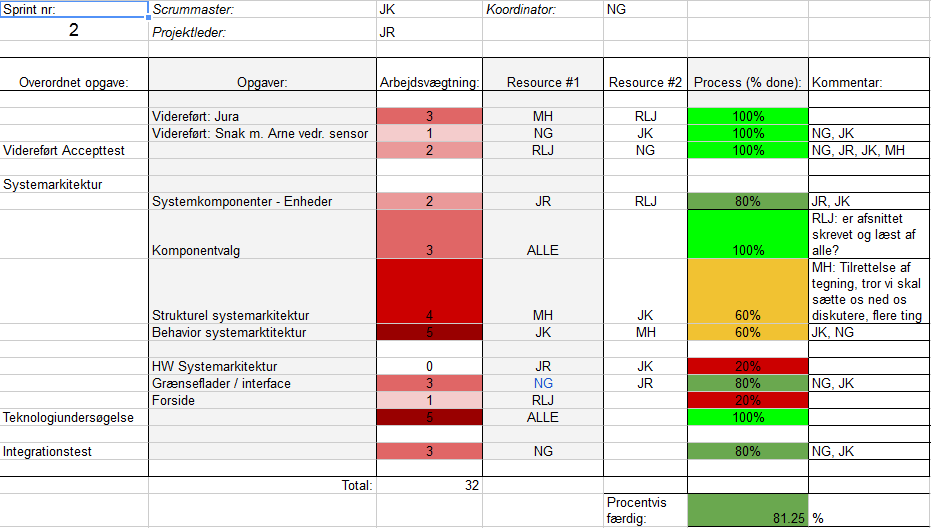
\includegraphics[width=0.9\textwidth]{billeder/SCRUM1}
\caption{Sprint 2}
\label{fig:SCRUM}
\end{figure}
Sprintet er afsluttet. De opgaver der ikke er færdige blev i det her eksempel videreført til sprint nummer tre. Billedet illustrerer også hvordan planlægningen er opbygget. Forklaring af statusfarver er vist på figur \ref{fig:SCRUM2}.
\begin{figure}[H]
\centering
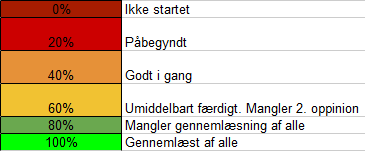
\includegraphics[width=0.5\textwidth]{billeder/SCRUM2}
\caption{Forklaring af sprint points}
\label{fig:SCRUM2}
\end{figure}
\subsection{V-model}
\begin{figure}[H]
\centering
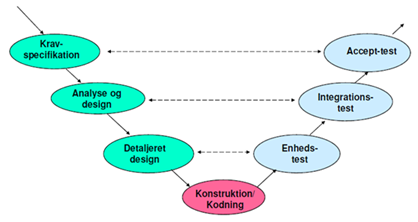
\includegraphics[width=0.5\textwidth]{billeder/vmodel}
\caption{V modellen}
\label{fig:vmodel}
\end{figure}
Vi har valgt at anvende V-modellen som udviklingsmodel. Dette muliggør iterative processer hvilket er optimalt for gruppens udviklingstil.